\documentclass[tikz, border=4pt]{standalone}
\usepackage{tikz}
\usepackage{tikz-cd}
\begin{document}
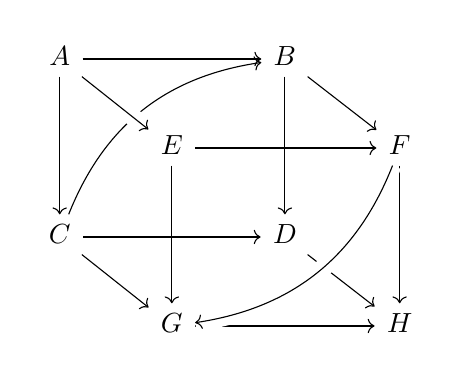
\begin{tikzpicture}[x=1cm, y=1cm]
  \node at (2.46,-1.94) {\pgfinterruptpicture%
  \begin{tikzcd}
  %first row
  A \ar[rr] \ar[dd] 
  & 
  & B \ar[dd] \ar[dr] \ar[from=ddll,bend left=30]
  & 
  \\
  %second row
  & E \ar[rr] \ar[dd] \ar[from=ul,crossing over]
  & 
  & F \ar[dd]
  \\
  %third row
  C \ar[rr] \ar[dr] 
  & 
  & D \ar[dr]
  & 
  \\
  %forth row
  & G \ar[rr] \ar[from=uurr,bend left=30,crossing over]
  & 
  & H
  \end{tikzcd}%
  \endpgfinterruptpicture};
\end{tikzpicture}
\end{document}
